\documentclass[a4paper, 14pt]{extarticle}

\usepackage[T2A]{fontenc} % поддержка русских букв
\usepackage{cmap} % копирование и поиск по русскому тексту
\usepackage[utf8]{inputenc}
\usepackage[english, russian]{babel}
\usepackage{geometry}

% sub figures / grids of pictures
\usepackage{subcaption} 
\usepackage{graphicx}
\graphicspath{{../img/}} % includegraphics path
\newcommand{\includegraphicsw}[2][1.]{\includegraphics[width=#1\linewidth]{#2}}
% pdf
\usepackage{pdfpages}
% tables
\let\oldtabular\tabular
\renewcommand{\tabular}[1][1.5]{\def\arraystretch{#1}\oldtabular}
\usepackage{multirow}
\usepackage{colortbl}
% \coloneqq
\usepackage{mathtools}
\usepackage{amssymb}
% math commands for convinience
\DeclareMathOperator{\argmin}{arg\,min}
% bold vectors
\newcommand{\vect}[1]{\boldsymbol{\mathbf{#1}}}
% listings
\usepackage{listings}
\lstset{
	basicstyle=\linespread{.95}\footnotesize\ttfamily\color{black},
	keywordstyle=\color{green!40!black},
	emphstyle=\bfseries\color{green!40!black},
	commentstyle=\itshape\color{purple!40!black},
	identifierstyle=\color{blue!30!black},
	showstringspaces=false,
	stringstyle=\color{orange},
	numbers=left,
	tabsize=2,
	breaklines=true,
	breakatwhitespace=true,
	language=C++
}


\begin{document}
	
	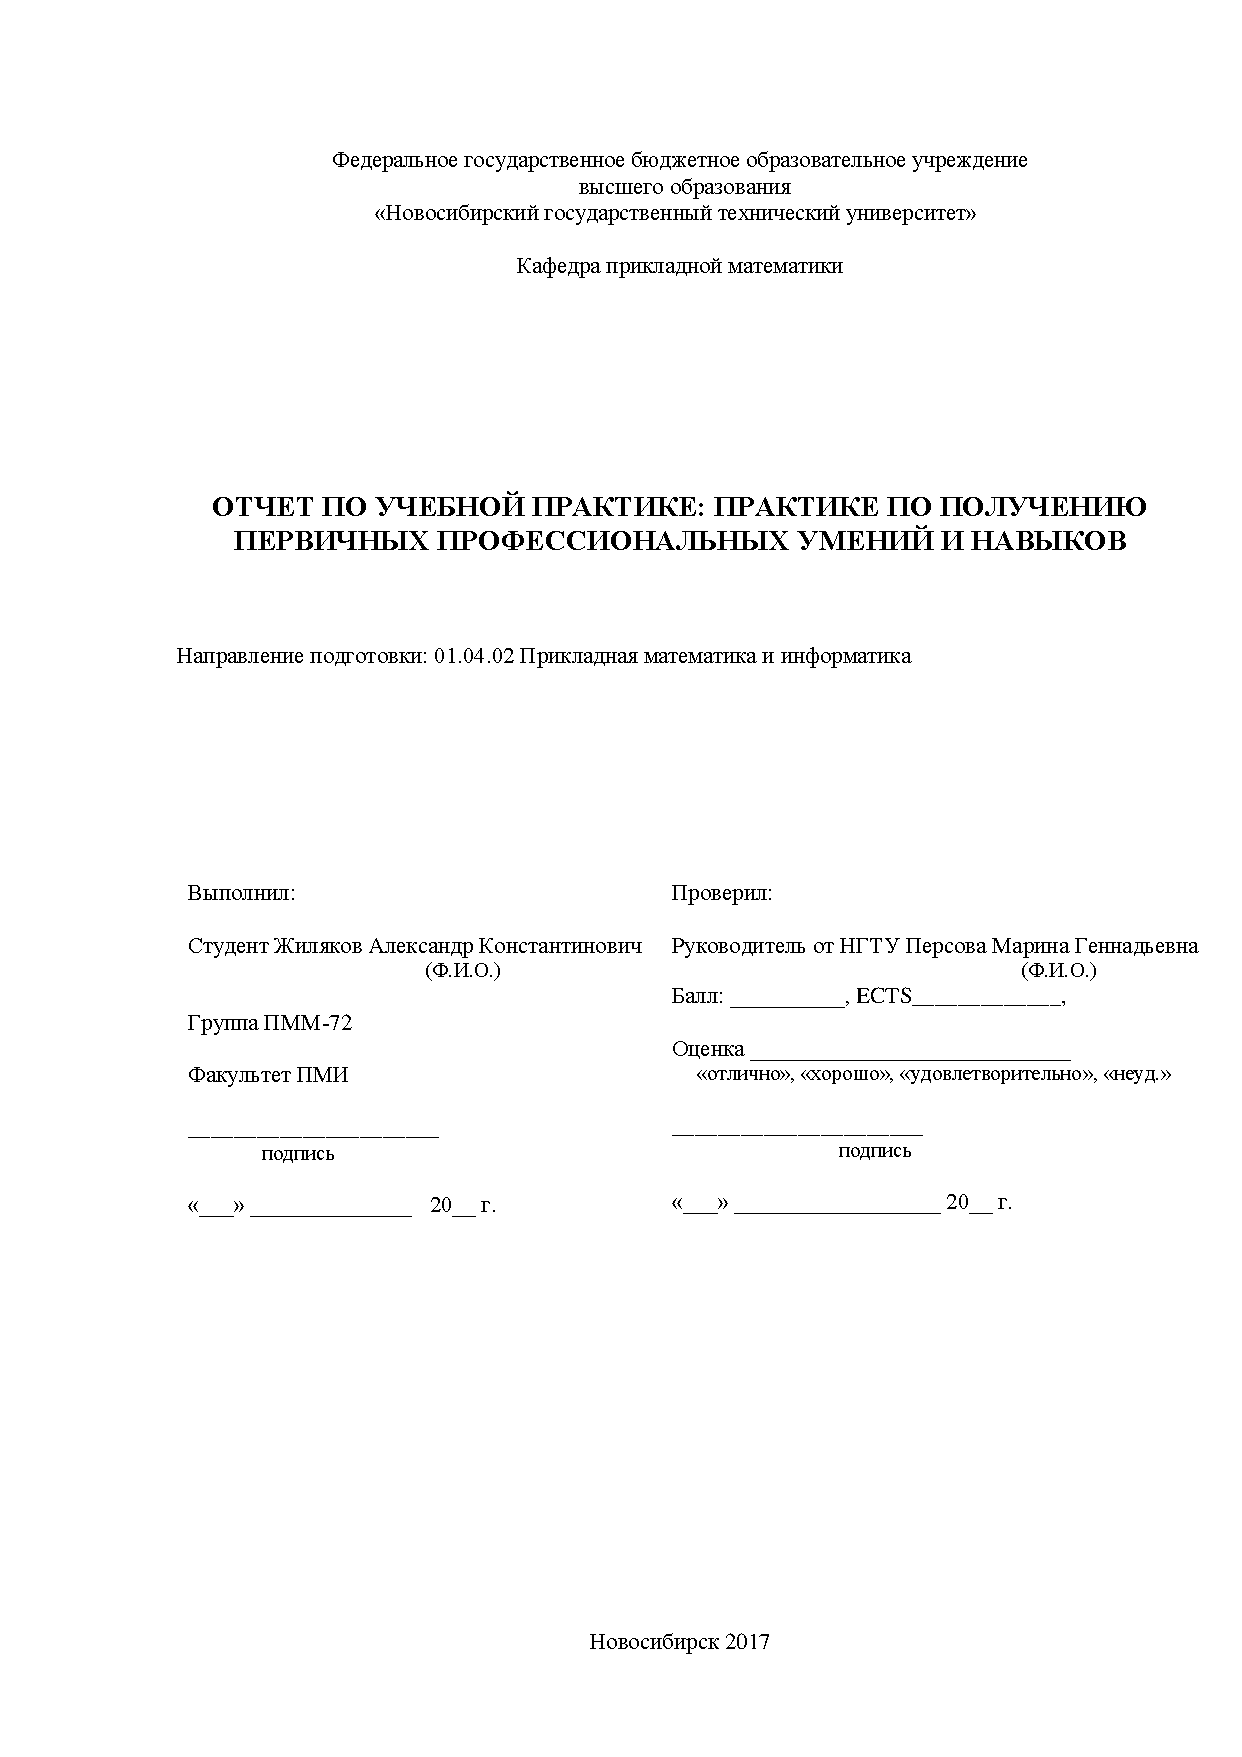
\includepdf{title.pdf}
	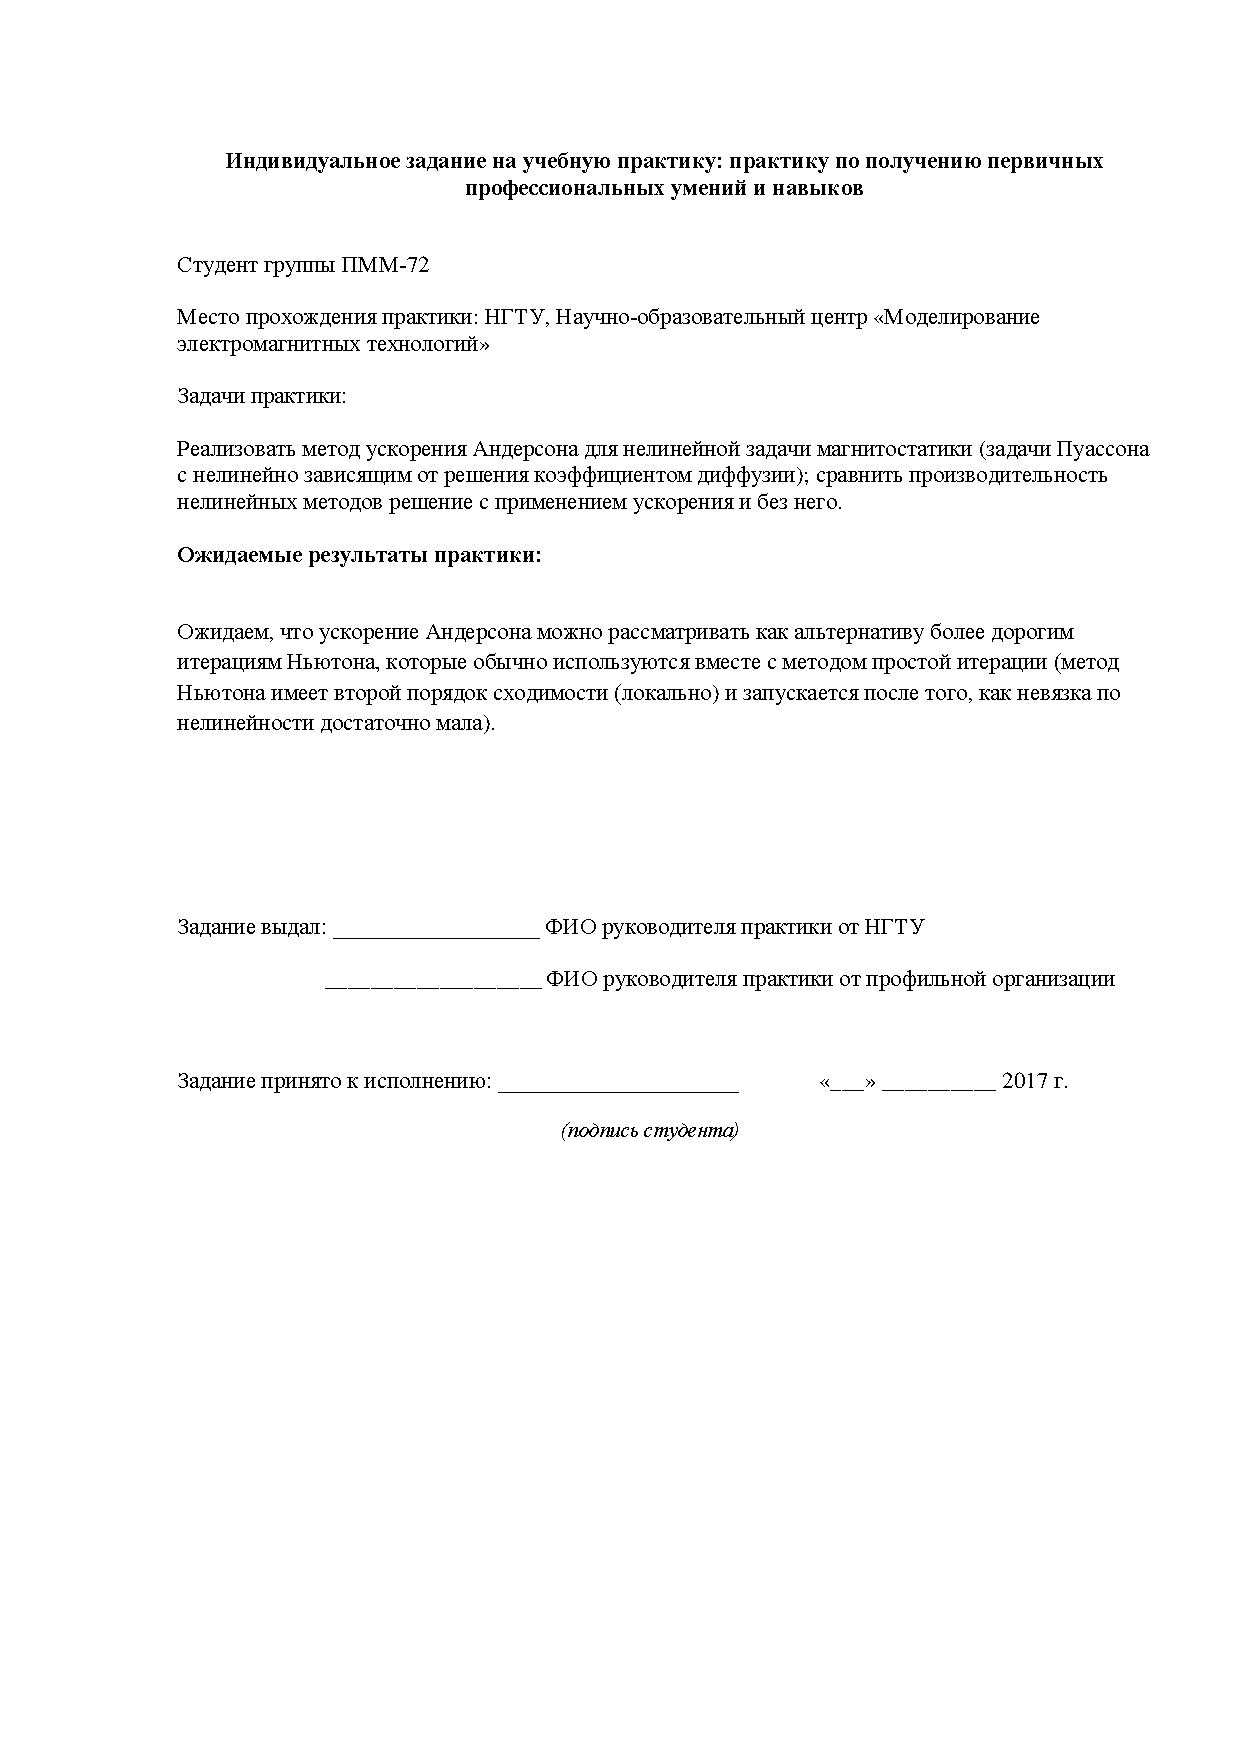
\includepdf{todo.pdf}
	
	\newgeometry{ 
		left=2cm, right=1.5cm, top=1.5cm, bottom=1.5cm,
		includefoot, heightrounded
	}
	
	\section{Описание задачи}
	
	\begin{figure}[b!]
		\centering
		\includegraphicsw[.6]{magnet.png}
		\caption{Сечение в плоскости $x\,O\,y$: железный магнит (выделен серым цветом), медные провода (выделены красным и синим)}
		\label{fig:magnet}
	\end{figure}
	
	Расчётная область представлена на рисунке~\ref{fig:magnet}. При заданной плотности тока $\vect J = (0, 0, J_z)$, $J_z \coloneqq \pm j \left[A\,m^{-2}\right]$, в проводах и магнитной проницаемости $\mu \left[N\,A^{-2}\right]$ железного тела, требуется найти результирующее поле магнитной индукции $\vect B \left[T\right]$.
	
	Физика данной задачи описывается системой Максвелла. Введём в рассмотрение вектор-потенциал~$\vect A$ через 
	$$
		\vect B = \nabla\times\vect A;
	$$
	тогда уравнения Максвелла $\nabla\times\frac{1}{\mu} \vect B = \vect J$, $\nabla\cdot\vect B = 0$ можно переписать в терминах вектор-потенциала
	$$
		\nabla\times\frac{1}{\mu}\nabla\times\vect A = \vect J.
	$$
	Предполагая, что магнит достаточно длинный в $z$-направлении и учитывая тот факт, что поле $\vect J$ имеет только одну ненулевую $z$-компоненту, $J_z = J_z(x, y)$, мы можем свести последнее уравнение к уравнению Пуассона
	\begin{equation}\label{poisson}
		-\nabla\cdot(\frac{1}{\mu}\nabla A_z) = J_z;
	\end{equation}
	из физических соображений задача~\eqref{poisson} оснащается однородными краевыми условиями Неймана (на нижней границе) и Дирихле (на остальной части). В результате КЭ дискретизации задача сведётся к решению линейной
	\begin{equation}\label{linear}
		\vect S\,\vect x = \vect b
	\end{equation}
	или нелинейной
	\begin{equation}\label{nonlinear}
		\vect S(\vect x)\,\vect x = \vect b
	\end{equation}
	системы уравнений в зависимости от того, каким образом магнитная проницаемость зависит от вектор-потенциала. 
	
	Представим магнитную проницаемость в виде $\mu = \mu_0\,\hat\mu$, где $\mu_0 \coloneqq 4\,\pi\,10^{-7} \left[N\,A^{-2}\right]$ есть проницаемость вакуума. Мы можем положить $\hat\mu_{\text{iron}} = 1000$ --- тогда~\eqref{poisson} сведётся к линейной системе~\eqref{linear}. В таком случае при изменении правой части уравнения меняться будет только масштаб решения (см. рисунок~\ref{fig:linearA}). 
	
	\begin{figure}
		\centering
		\begin{subfigure}{.45\linewidth}
			\centering
			\includegraphicsw{l06.png}
			\caption{$|J_z| = 10^6\,A\,m^{-2}$}
		\end{subfigure}%
		\hfill
		\begin{subfigure}{.45\linewidth}
			\centering
			\includegraphicsw{l11.png}
			\caption{$|J_z| = 10^{11}\,A\,m^{-2}$}
		\end{subfigure}
		\caption{Конечно элементные интерполянты вектор-потенциала~$A_z$, полученные при решении линейной задачи~\eqref{linear}}
		\label{fig:linearA}
	\end{figure}
	
	В действительности же $\hat\mu_{\text{iron}}$ нелинейно зависит $\vect B$ (см. рисунок~\ref{mu}) --- $\mu_{\text{iron}} = \mu_{\text{iron}}(||\vect B|| = ||\nabla A_z||)$. При таком раскладе~\eqref{poisson} сведётся к нелинейной системе~\eqref{linear}. Далее мы рассмотрим методы решения нелинейных систем. 
	
	\begin{figure}[b!]
		\centering
		\begin{subfigure}{.45\linewidth}
			\centering
			\includegraphicsw{interp.pdf}
			\caption{$\hat\mu_{\text{iron}} = \hat{\mu}_{\text{iron}}(||\vect B||)$}
		\end{subfigure}%
		\hfill
		\begin{subfigure}{.45\linewidth}
			\centering
			\includegraphicsw{extrap.pdf}
			\caption{Часть с экстраполяцией}
		\end{subfigure}
		\caption{Интерполянт для магнитной проницаемости, построенный по реальным данным}
		\label{mu}
	\end{figure}
	
	\section{Ускорение Андерсона}
	
	Пусть требуется решить нелинейную задачу
	\begin{equation}\label{f}
		\vect f(\vect x) = 0.
	\end{equation}
	От задачи поиска корня~\eqref{f}, записанной в терминах оператора невязки~${\vect f : \mathbb R^n \rightarrow \mathbb R^n}$, можно перейти к эквивалентной задаче поиска фиксированной точки
	\begin{equation}\label{g}
		\vect x = \vect g(\vect x),
	\end{equation}
	записанной в терминах оператора итераций~$\vect g$. (Сделать это можно, например, положив~$\vect g(\vect x) \coloneqq \vect x - \gamma\,\vect f(\vect x)$.)
	
	Выбрав начальное приближение~$\vect x^{(0)}$, для решения~\eqref{g} можно применить \textbf{метод простой итерации}
	\begin{equation}\label{fp}
		\vect x^{(k+1)} = \vect g(\vect x^{(k)}).
	\end{equation}
	
	Для ускорения сходимости~\eqref{fp} можно предложить следующую идею. Будем искать новое приближение используя $(m + 1)$ предыдущих приближений:
	\begin{equation}\label{mixing}
		\vect x^{(k+1)} = \sum_{i=0}^m \alpha_i\,\vect g(\vect x^{(k-i)}).
	\end{equation}
	Метод~\eqref{mixing} будет состоятельным тогда и только тогда, когда 
	\begin{equation*}
		\sum_{i=0}^m \alpha_i = 1.
	\end{equation*}
	Коэффициенты~$\alpha_i$ будем искать решая задачу минимизации
	\begin{equation}\label{min}
		\vect\alpha = \underset{\sum_{i=0}^m \alpha_i = 1}{\argmin} \left\lVert \sum_{i=0}^m \alpha_i\,\vect f(\vect x^{(k-i)}) \right\lVert_2.
	\end{equation}
	
	Представим коэффициенты~$\alpha_i$ в виде
	\begin{equation}\label{beta}
		\begin{aligned}
			\alpha_0		&= 1 - \beta_1, \\
			\alpha_1		&= \beta_1 - \beta_2, \\
			\vdots			& \\
			\alpha_{m-1}	&= \beta_{m-1} - \beta_m, \\
			\alpha_m		&= \beta_m;
		\end{aligned}
	\end{equation}
	тогда задачу минимизации с ограничениями~\eqref{min} можно переписать как задачу минимизации без ограничений --- свести её к \textbf{задаче о наименьших квадратах}
	\begin{equation}\label{lsq}
		\begin{aligned}
			\vect\beta 
				&= \underset{\vect\beta \in \mathbb R^m}{\argmin} \left\lVert \vect f(\vect x^{(k)}) - \sum_{i=1}^{m} \beta_i\,(\vect f(\vect x^{(k-i)}) - \vect f(\vect x^{(k-i+1)})) \right\lVert_2 \\
				&= \underset{\vect\beta \in \mathbb R^m}{\argmin} \left\lVert \vect f(\vect x^{(k)}) - \vect F\,\vect\beta \right\lVert_2, 
		\end{aligned}
	\end{equation}
	которая эквивалентна решению системы
	\begin{equation}\label{normal}
		\left(\vect F^T\,\vect F\right)\,\vect\beta = \vect F^T\,\vect f(\vect x^{(k)}).
	\end{equation}
	Здесь через $\vect F$ обозначена матрица из разностей нелинейных невязок
	$$
		\vect F \coloneqq \begin{bmatrix}
			\vect f(\vect x^{(k)}) - \vect f(\vect x^{(k-1)}) & | \dots | & \vect f(\vect x^{(k-m+1)}) - \vect f(\vect x^{(k-m)})
		\end{bmatrix} \in \mathbb R^{m \times n}.
	$$
	
	Таким образом, \textbf{метод ускорения Андерсона} (или метод смешивания Андерсона) для задачи~\eqref{fp} записывается в следующем виде. Используя информацию об ${(m + 1)}$ предыдущих приближениях, найти новое приближение в виде
	$$
		\vect x^{(k+1)} = \sum_{i=0}^m \alpha_i\,\vect g(\vect x^{(k-i)}),
	$$  
	где коэффициенты~$\vect\alpha$ выражаются через коэффициенты~$\vect\beta$~\eqref{beta}, которые находятся из решения нормальной системы~\eqref{normal}.
	
	Обычно количество смешиваний (размер матрицы системы~\eqref{normal})~$m$ выбирается в диапазоне 10\,--\,50, $m \ll n$, и для составления матрицы требуется~$O(n)$ операций на каждой нелинейной итерации метода~\eqref{fp}; для небольшой системы достаточно использовать LU факторизацию / метод исключения Гаусса c partial pivoting (используется в нашей реализации)\footnotemark{}. Заметим, что в обычном методе~\eqref{fp} мы исполняем как минимум~$O(n)$ операций на каждой нелинейной итерации, реассемблируя конечно-элементную матрицу, так что ускоренный метод~$\eqref{mixing}$ асимптотически эквивалентен методу~\eqref{fp} в терминах необходимых операций и затрат ОЗУ на каждой нелинейной итерации. 
	
	\footnotetext{
		Другой вариант (белее подходящий с точки зрения устойчивости при работе в конечной арифметике) решения задачи наименьших квадратов~\eqref{lsq} --- метод ортогональных преобразований с использованием отражений Хаусхолдера. 
	}
	
	Выбор коэффициентов в~\eqref{min} обусловлен следующим наблюдением. Предположим, что приближения~$\vect x^{(k)}, \dots, \vect x^{(k-m+1)}$ достаточно близки друг к другу и дефекты~$|| \vect x^{(i)} - \vect g(\vect x^{(i)}) ||_2$ достаточно малы. Тогда
	\begin{equation}\label{linres}
		\begin{aligned}
			\vect f(\vect x^{(k+1)}) 
			&= \vect f\left( \sum_{i=0}^m \alpha_i\,\vect g(\vect x^{(k-i)}) \right) \\
			&= \vect f\left( \sum_{i=0}^m \alpha_i\,\vect x^{(k-i)} - \sum_{i=0}^m \alpha_i\,\left( \vect x^{(k-i)} - \vect g(\vect x^{(k-i)}) \right) \right) \\
			&\approx \vect f\left( \sum_{i=0}^m \alpha_i\,\vect x^{(k-i)} \right) \\
			&= \vect f\left( \vect x^{(k)} - \sum_{i=1}^m \beta_i\,\left( \vect x^{(k-i+1)} - \vect x^{(k-i)} \right) \right) \\
			&\approx \vect f(\vect x^{(k)}) - \sum_{i=1}^m \beta_i\,\vect f'(\vect x^{(k)})\,\left( \vect x^{(k-i+1)} - \vect x^{(k-i)} \right) \\
			&\approx \vect f(\vect x^{(k)}) - \sum_{i=1}^m \beta_i\,\left( \vect f(\vect x^{(k-i+1)}) - \vect f(\vect x^{(k-i)}) \right) \\
			&=\sum_{i=0}^m \alpha_i\,\vect f(\vect x^{(k-i)}). 
		\end{aligned}
	\end{equation}
	
	Таким образом, решая~\eqref{min} в методе ускорения Андерсона мы надеемся минимизировать невязку $(k+1)$-го приближения. Поэтому метод ускорения Андерсона иногда называют нелинейным аналогом GMRES.
	
	\section{Численные результаты}
	
	Для задачи~\eqref{nonlinear} оператор невязки имеет вид
	$$
		\vect f(\vect x) \coloneqq \vect b - \vect S(\vect x)\,\vect x.
	$$
	В качестве оператора итераций можно выбрать, например, 
	\begin{equation}\label{picard}
		\vect g(\vect x) \coloneqq \vect S^{-1}(\vect x)\,\vect b
	\end{equation}
	или
	\begin{equation}\label{newton}
		\vect g(\vect x) \coloneqq \vect x - \left[ \vect f'(\vect x) \right]^{-1} \vect f(\vect x).
	\end{equation} 
	Метод~\eqref{picard} называется \textbf{методом Пикарда} (так же методом простой итерации или упрощённым методом Ньютона), а метод~\eqref{newton} --- \textbf{методом Ньютона}.
	
	На каждой итерации обоих методов необходимо вычислять результат действия матрицы, обратной к дискретному эллиптическому оператору (симметричная положительно определённая матрица); мы делаем это с помощью метода сопряжённых градиентов с неполным $LDL^T$ переобуславливателем. Метод Ньютона~\eqref{newton} c вычислительной точки зрения дороже, чем~\eqref{picard}, потому что он требует вычисления матрицы Якоби; кроме того метод Ньютона имеет \textit{локальный} квадратичный порядок сходимости.
	
	Для решения больших нелинейных систем обычно используют следующий подход: обрушают нелинейную невязку с помощью относительно дешёвого метода, --- например,~\eqref{picard}, --- а затем запускают метод Ньютона.
	
	В данной работе мы вместо метода Ньютона для ускорения сходимости использовали более дешёвый с вычислительной точки зрения метод смешивания Андерсона\footnotemark{} для ускорения сходимости метода Пикарда~\eqref{picard}.
	
	\footnotetext{
		Ускорение Андерсона подходит для любого метода, записанного в форме~\eqref{g} --- в том числе и для метода Ньютона~\eqref{newton}. В данной работе мы рассматриваем только производительность ускоренного метода Пикарда~\eqref{picard}.
	} 

	На практике отображение~$\vect g$ редко является сжимающим, поэтому для обрушения невязки мы использовали метод Пикарда с релаксацией
	\begin{equation}\label{wpicard}
		\vect g_\omega(\vect x) \coloneqq \omega\,\vect S^{-1}(\vect x)\,\vect b + (1 - \omega)\,\vect x,
	\end{equation}
	$0 < \omega \le 1$. Здесь параметр~$\omega$ выбирался адаптивно --- начиная с единичного значения, мы делили его на 10 до тех пор, пока норма новой нелинейной невязки не становилась меньше текущей. Метод~\eqref{wpicard} дороже~\eqref{picard}: на одной итерации невязку приходится вычислять несколько раз.
	
	\begin{table}\centering
		\caption{Количество итераций и время работы для разных нелинейных методов решения системы~\eqref{nonlinear}} 
		\label{tab:res}
		\begin{tabular}[2]{ | c | c | c | >{\columncolor[gray]{0.9}}c | >{\columncolor[gray]{0.9}}c | >{\columncolor[gray]{0.9}}c | c | }
			\hline
			Плотность тока $|J_z|$, $\left[A\,m^{-2}\right]$ & $10^6$ & $10^7 $& $10^8$ & $10^9$ &$10^{10}$ & $10^{11}$ \\
			\hline
			\multirow{2}{*}{Метод Пикарда~\eqref{picard}} 
			& 1 & 6 & --- & --- & 203 & 7 \\
			& 0.4\,s & 1.3\,s & --- & --- & 25.2\,s & 1\,s \\
			\hline
			\multirow{2}{*}{Метод Пикарда с релаксацией~\eqref{wpicard}} 
			& 1 & 6 & 84 & 70 & 164 & 7 \\
			& 0.5\,s & 2\,s & 71\,s & 52.4\,s & 54.3\,s & 2.6\,s \\
			\hline
			\multirow{2}{*}{Ускорение Андерсона~\eqref{mixing}} 
			& 1+0 & 0+4 & 22+20 & 21+21 & 35+6 & 4+2 \\
			& 0.7\,s & 1\,s & 20\,s & 14.5\,s & 11.4\,s & 1.9\,s \\
			\hline
		\end{tabular}
	\end{table} 
	
	Результаты приведены в таблице~\ref{tab:res}. Использовались линейные Лагранжевы элементы первого порядка (сетка изображена на рисунке~\ref{fig:magnet}, 362 степени свободы). Критерий остановки: $\vect f(\vect x^{(k)}) < 10^{-8}$. Для метода смешивания Андерсона~$k = i + j$ означает $i$ итераций Пикарда с \textit{релаксацией}\footnotemark{} ($\vect f(\vect x^{(i)}) < 10^{-4}$) и $j$ \textit{ускоренных} итераций Пикарда. Мы использовали количество смешиваний~$m = 10$.
	
	\footnotetext{
		Из~\eqref{linres} видно, что ускорение Андерсона применимо при определённых предположениях, поэтому для обрушения невязки мы использовали метод Пикарда с релаксацией. 
	}    
	
	Из таблицы видно, что степень «сложности» нелинейной задачи сильно зависит от применяемой плотности тока: при плотности вне промежутка~$10^8\,--\,10^{10} \left[A\,m^{-2}\right]$ оказывается достаточным использовать простой метод Пикарда; внутри промежутка метод оказывается неработоспособным.
	
	Применение метода Пикарда с релаксацией позволяет решить задачу, однако временные затраты получается колоссальными (с учётом скромного размера системы, $n = 362$). Из таблицы видно, что применение ускорения Андерсона позволяет методу сойтись в $>3$ раза быстрее. 
	
	Решения представлены на рисунке~\ref{fig:nonlinearA}.

	\begin{figure}
		\centering
		\begin{subfigure}{.42\linewidth}
			\centering
			\includegraphicsw{a_nonlinear_6.png}
		\end{subfigure}%
		\hfill
		\begin{subfigure}{.42\linewidth}
			\centering
			\includegraphicsw{a_nonlinear_7.png}
		\end{subfigure}%
		\par\bigskip
		\begin{subfigure}{.42\linewidth}
			\centering
			\includegraphicsw{a_nonlinear_8.png}
		\end{subfigure}%
		\hfill
		\begin{subfigure}{.42\linewidth}
			\centering
			\includegraphicsw{a_nonlinear_9.png}
		\end{subfigure}%
		\par\bigskip
		\begin{subfigure}{.42\linewidth}
			\centering
			\includegraphicsw{a_nonlinear_10.png}
		\end{subfigure}%
		\hfill
		\begin{subfigure}{.42\linewidth}
			\centering
			\includegraphicsw{a_nonlinear_11.png}
		\end{subfigure}
		\caption{Конечно элементные интерполянты вектор-потенциала~$A_z$, полученные при решении нелинейной задачи~\eqref{nonlinear}: $|J_z| = 10^6, 10^7, \dots, 10^{11}\,A\,m^{-2}$}
		\label{fig:nonlinearA}
	\end{figure}
	
	\section{Исходный текст программы}
	
	\subsection{NonlinearSolvers.hpp}
	
	Модуль с имплементацией общего нелинейного решателя в форме~\eqref{fp} и метода ускорения Андерсона~\eqref{mixing}.
	
	\lstinputlisting{NonlinearSolvers.hpp}
	
	\subsection{user.cpp}
	
	Модуль с имплементацией конечно-элементного решения линейной и нелинейной задач магнитостатики~\eqref{poisson}.
	
	\lstinputlisting{user.cpp}
	
\end{document}


